\documentclass{article}

\usepackage[utf8]{inputenc}
\usepackage{tikz}

\title{Memory Allocator}

\begin{document}
\maketitle
\thispagestyle{empty}
\newpage

\tableofcontents
\thispagestyle{empty}
\newpage

\setcounter{page}{1}

problembeskrivning och föreslagen lösning, antaganden som inte nämnts i uppgiften, UML-diagram för minneshanterare och andra komponenter som använder den, grafer med exekveringstid för olika valda scenarion, sammanfattning som förklarar resultat och analyserar (i allmänhet) användning av minnesallokatorer i spelprojekt (t.ex förklarar vilka situationer i ett spel som gynnas av att använda varje typ av allokator)

\section{Memory manager}
Beskrivning av minneshanterare, UML (som även visar hur tester använder den) osv

\section{Pool allocator}
Sometimes, objects that need to be allocated are of the same (or similar) size, but may also be deallocated independently. For this usage a pool allocator is very suitable because it supports deallocating in an arbitrary order without fragmentation. This is because allocation is performed in chunks, which means that the size of an allocation is always the same and by extension an allocation will never fail provided that there is at least one free chunk in the pool.

Storing a number of blocks of a certain size is not enough -- we also need to keep track of which ones are available to be allocated. Our housekeeping is done using a linked list of chunks that uses the unallocated block for its data by storing a pointer to the next free block, see figure~\ref{fig:pool_free_blocks}. When allocating, an all-or-nothing approach is used in the sense that an entire block is allocated -- never parts of one. Of course, the user may choose to store less data in the given block, but the unused data is still considered to be allocated.

\begin{figure}[h]
    \centering
    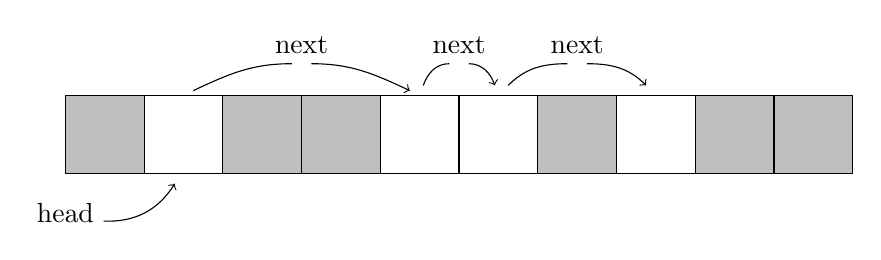
\begin{tikzpicture}
        % empty blocks
        \draw (1,0) rectangle (2,1);
        \draw (4,0) rectangle (5,1);
        \draw (5,0) rectangle (6,1);
        \draw (7,0) rectangle (8,1);
        % occupied blocks
        \filldraw[fill=gray!50,draw=black] (0,0) rectangle (1,1);
        \filldraw[fill=gray!50,draw=black] (2,0) rectangle (3,1);
        \filldraw[fill=gray!50,draw=black] (3,0) rectangle (4,1);
        \filldraw[fill=gray!50,draw=black] (6,0) rectangle (7,1);
        \filldraw[fill=gray!50,draw=black] (8,0) rectangle (9,1);
        \filldraw[fill=gray!50,draw=black] (9,0) rectangle (10,1);
        % declare points for arrow start/end and text positions
        \node at (0,-0.5) (head) {head};
        \node at (1.5,0) (b1_lower) {};
        \node at (1.5,1) (b1_upper) {};
        \node at (3,1.4) (n1) {};
        \node at (4.5,1) (b4) {};
        \node at (5,1.4) (n2) {};
        \node at (5.5,1) (b5) {};
        \node at (6.5,1.4) (n3) {};
        \node at (7.5,1) (b7) {};
        % draw arrows
        \draw[->,bend right] (head) to (b1_lower);
        \draw[->] (b1_upper) to[out=25,in=180] (n1) to[out=0,in=155] (b4);
        \draw[->] (b4) to[out=70,in=180] (n2) to[out=0,in=110] (b5);
        \draw[->] (b5) to[in=180] (n3) to[out=0] (b7);
        % next labels
        \foreach \p in {n1,n2,n3}
            \node[above] at (\p) {next};
    \end{tikzpicture}
    \caption{Free block tracking. A pointer inside the pool allocator keeps track of the first block. Each block uses the storage to store a pointer to the next empty block, thereby forming a linked list. The tail element stores a null pointer to indicate end of list.}
    \label{fig:pool_free_blocks}
\end{figure}

Allocation and deallocation are very simple with the pool allocator and is performed in $O(1)$ complexity. Allocation is a matter of consuming a free block and making sure that the list of free blocks is properly updated. We do this by allocating the first free block and setting the head of the list to be the second free block. Similarly, deallocation is done by putting the returned block at the head of the list and connecting it to the previous head. See figures~\ref{fig:pool_allocation} and~\ref{fig:pool_deallocation} for details on how this is done.

\textbf{två figurer som visar hur allokering och avallokering uppdaterar listan}

\section{Stack allocator}
Beskrivning av stackallokatorn

\section{Tests}
Beskriver hur testerna fungerar och vad de gör, vad de mäter osv

\section{Results}
Graferna med förklarande text. Vet inte vad mer som går in egentligen

\section{Conclusion}
Förklara resultat, konstatera att minnesallokatorerna gör stor skillnad gentemot allokeringen som tillhandahålls av OS.
\end{document}
